\documentclass[a4paper,11pt,fleqn]{article}%fleqn pour aligner les equations à gauche
\usepackage{graphicx}
\usepackage[utf8]{inputenc}  
\usepackage[T1]{fontenc}
\usepackage{lscape}

\usepackage{tgheros,textcomp}%Police Arial
\renewcommand{\familydefault}{\sfdefault}

%\setlength{\mathindent}{0pt}%indentation dans math = 0

\usepackage[top = 1cm, bottom = 2cm, left = 1cm, right = 1cm]{geometry}
\usepackage{titlesec}
%\setcounter{secnumdepth}{4}
\usepackage{xcolor}
\usepackage{amssymb} %double flèche de réaction
\usepackage{mathrsfs}%farraday
\usepackage{xtab}%tableau sur plusieurs pages
\usepackage{esvect}%grands vecteurs

\usepackage[version=4]{mhchem} %equations chimiques

\usepackage{array}
\usepackage{chemfig}
\usepackage{multirow}
%\usepackage{sectsty}

\usepackage{caption}
\usepackage{adjustbox}
\usepackage[labelformat=simple]{subfig}
\usepackage{float}


\usepackage{amsmath}
\usepackage{amssymb}
\usepackage[cal=boondoxo]{mathalfa} 
\usepackage{enumitem}
\usepackage{lastpage}
\usepackage{tcolorbox}
\usepackage{siunitx}
\usepackage[european, straightvoltages, RPvoltages]{circuitikz}
\usepackage{tikz}
\usetikzlibrary{shapes.geometric}
\usetikzlibrary{calc}
\usetikzlibrary{automata,positioning}
\usepackage{multicol}
\usepackage{eqnarray}
\usepackage{tabularx,colortbl}%colorer fond cellules

\sisetup{
	detect-all,
	output-decimal-marker={,},
	group-minimum-digits = 3,
	group-separator={~},
	number-unit-separator={~},
	inter-unit-product={~}
} %setup pour SIunitx

\usepackage{listings}%pour insérer le code python
\definecolor{codegreen}{rgb}{0,0.6,0}
\definecolor{codegray}{rgb}{0.5,0.5,0.5}
\definecolor{codepurple}{rgb}{0.58,0,0.82}
\definecolor{backcolour}{rgb}{0.95,0.95,0.92}


\titleformat{\section}
{
\vspace{.8ex}%
\normalfont \bfseries \large}
{\thesection.}{.5em}{\bfseries}

\renewcommand{\thesection}{\arabic{section}}
\titlespacing{\section}{0pt}{1em}{.5em}
\renewcommand{\thesubsection}{\hspace{1cm}\alph{subsection}.}
\renewcommand\thesubfigure{\textbf{Document \arabic{subfigure} :}}

\title{\vspace{-1cm}\large 
	\begin{tabular}{|>{\centering}m{5cm}|>{\centering}m{8cm}|>{\centering\arraybackslash}m{4cm}|}
		\hline
		Activité Expérimentale 1 & \textbf{\textsc{Evolution spontanée d'un système chimique}} &  Chapitre 7 \\
		\hline
\end{tabular}}
\date{}

\newpagestyle{mystyle}{%
	\setfoot{ROSALIE}{\thepage\,$|$\,\pageref{LastPage}}{}
}
\renewpagestyle{plain}{%
	\setfoot{ROSALIE}{\thepage\,$|$\,\pageref{LastPage}}{}
}

\pagestyle{mystyle}

\newenvironment{itemize*}%
{\begin{itemize}[label=$-$,labelindent=0pt, leftmargin=*,topsep=0pt]%
		\setlength{\itemsep}{0pt}%
		\setlength{\parskip}{0pt}}%
	{\end{itemize}}

\newenvironment{itemize**}%
{\begin{itemize}[label=,labelindent=0pt, leftmargin=*,topsep=0pt]%
		\setlength{\itemsep}{0pt}%
		\setlength{\parskip}{0pt}}%
	{\end{itemize}}

\renewcommand{\arraystretch}{1.5}

  
\begin{document}
\maketitle
\vspace{-2.5cm}

\textbf{Objectifs : } Afin d'optimiser le rendement de leurs processus de fabrication, les industries chimiques doivent être capables de déterminer si une réaction chimique est totale ou non. \textbf{Comment vérifier le caractère total ou non d'une transformation chimique ? Quelle est la relation entre les concentrations des espèces chimiques à l'équilibre ?}
\section{Transformation totale ou non}
On souhaite savoir si la réaction entre les ions thiocyanate et les ions fer(III) est totale ou non.\\
\noindent
\fbox{
\begin{minipage}[t][6cm][t]{.45\textwidth}
\textbf{Document 1 : Équation de la réaction}\\
Le thiocyanate de potassium \ce{KSCN} dissout en solution, libère des ions \ce{K+(aq)} et thiocyanate \ce{SCN-(aq)}. Ces derniers réagissent avec les ions fer (III), \ce{Fe^{3+}(aq)} selon la réaction d'équation :
$$\ce{Fe^{3+}(aq) + SCN-(aq) <=> FeSCN^{2+}(aq)}$$
La réaction entre les ions thiocyanate \ce{SCN-(aq)} et les ions fer \ce{Fe^{3+}(aq)} est utilisée pour fabriquer du faux sang.
\end{minipage}}
\fbox{\begin{minipage}[t][6cm]{.5\textwidth}
\textbf{Document 2 : Coloration des solutions}\\
- Solution sans ions \ce{Fe^{3+}(aq)}, ni \ce{FeSCN^{2+}(aq)} : incolore\\
- Solution contenant des ions  \ce{Fe^{3+}(aq)} : jaune pâle\\
- Solution contenant des ions  \ce{FeSCN^{2+}(aq)} : rouge
\end{minipage}}

\noindent
\fbox{
\begin{minipage}[t][3.5cm]{.5\textwidth}
\textbf{Document 3 : Définitions}\\
 \underline{Transformation totale :} une transformation chimique est totale si au moins l'un des réactifs a été entièrement consommé.\\
\underline{Transformation non totale :} une transformation chimiques est non totale si tous les réactifs sont encore présents à la fin de la réaction.
\end{minipage}}
\noindent
\fbox{
\begin{minipage}[t][3.5cm][t]{.45\textwidth}
\textbf{Document 4 : Matériel nécessaire}\\
- Solution de (\ce{K+(aq)} ; \ce{SCN-(aq)}) à $c$ = \SI{0,005}{\mole \per \liter} en soluté \ce{KSCN} apporté\\
- Solution de (\ce{Fe^{3+}(aq)} ; \ce{3Cl-(aq)}) à $c$ = \SI{0,005}{\mole \per \liter} en soluté \ce{FeCl3} apporté\\
- Trois béchers de \SI{150}{\milli \liter}, numérotés de 1 à 3\\
- Éprouvettes graduées de \SI{50}{\milli \liter} et \SI{5}{\milli \liter}
\end{minipage}}

\begin{enumerate}
	\item Dans le bécher 1, introduire environ \SI{50}{\milli \liter} de solution de chlorure de fer(III) puis ajouter environ \SI{5}{\milli \liter} de solution de thiocyanate de potassium. Décrire la couleur de la solution.
	\item Verser de nouveau environ \SI{5}{\milli \liter} de solution de thiocyanate de potassium dans ce même bécher. Décrire l'évolution de la couleur.
	\item Répartir la solution obtenue dans les béchers 1, 2 et 3. Le bécher 1 sert de témoin. Verser de nouveau environ \SI{5}{\milli \liter} de solution de thiocyanate de potassium dans le bécher 2. Expliquer l'évolution de la couleur.
	\item Verser environ \SI{5}{\milli \liter} de solution chlorure de fer(III) dans le bécher 3. Justifier l'évolution de la couleur.
	\item Conclure quant au caractère total ou non de la transformation chimique du bécher 1.
	\section{Constante d'équilibre}
On souhaite déterminer la constante d'équilibre de la réaction entre les ions thiocyanate et les ions fer(III).
\begin{enumerate}
	\item Remplir le tableau d'avancement ci-dessous en utilisant les notations suivantes :
	\begin{itemize}
		\item quantité de matière d'ion fer \ce{Fe^{2+}} dans l'état initial : $n_{F,i}$
		\item quantité de matière d'ion fer \ce{SCN-} dans l'état initial : $n_{T,i}$
		\item avancement à l'état final : $x_f$
	\end{itemize}
\end{enumerate}
\end{enumerate}
\begin{tabular}{|>{\centering}m{3cm}|>{\centering}m{3cm}|>{\centering}m{3cm}|>{\centering}m{3cm}|>{\centering\arraybackslash}m{3cm}|}
\hline \multicolumn{2}{|c|}{\rule[1cm]{0cm}{0cm}}&\multicolumn{3}{|>{\centering}c|}{}\\
\hline État initial & $x=0$ & & &\\
\hline État final & $x_f$ & & &\\
\hline 
\end{tabular}
\begin{enumerate}[resume]
	\item Surligner la case du tableau correspondant à la quantité de matière en ion \ce{FeSCN^{2+}(aq)} à l'état final
	\item Montrer que l'avancement final est donné par la formule : $$x_f = [\ce{FeSCN^{2+}(aq)}]_f \times V$$ avec $[\ce{FeSCN^{2+}(aq)}]_f$ la concentration finale obtenue en ion \ce{FeSCN^{2+}}.
\end{enumerate}
Pour déterminer l'avancement final et connaître ainsi les quantités de matière des réactifs et des produits, il faut déterminer $[\ce{FeSCN^{2+}(aq)}]_f$. Pour cela, on utilise la courbe d'étalonnage en fonction de la concentration en ion \ce{FeSCN^{2+}}.\\

\noindent \fbox{
\begin{minipage}{.98\textwidth}
\textbf{Document 5 : Spectre UV-Visible obtenu pour une solution d'ions\ce{FeSCN^{2+}}}
\begin{center}
	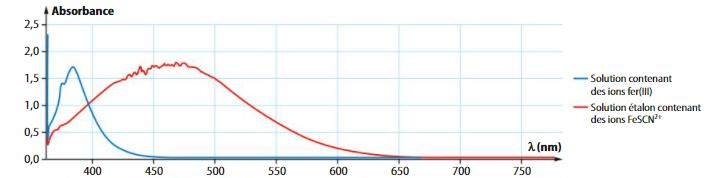
\includegraphics[scale=.75]{Ressources/TSPE_C7_AE1_Fig1.png}
\end{center}
\end{minipage}
}

\noindent \fbox{
\begin{minipage}{.98\textwidth}
\textbf{Document 6 : Courbe d'étalonnage}
\begin{center}
	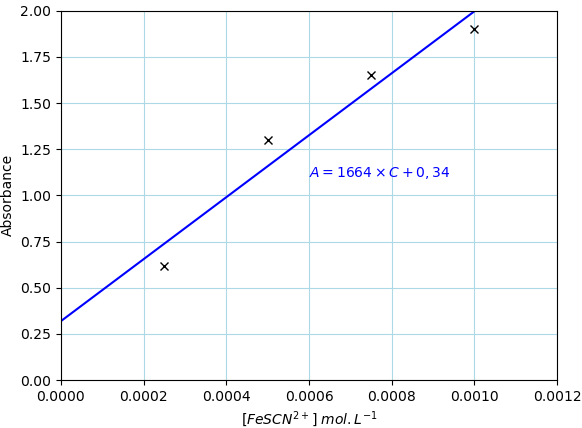
\includegraphics[scale=.7]{Ressources/TSPE_C7_AE1_Fig2.png}
\end{center}
\end{minipage}
}

\noindent \fbox{
\begin{minipage}{.98\textwidth}
\textbf{Document 7 : Quotient de réaction}\\
On considère une transformation chimique en solution aqueuse modélisée par équation du type : $$\ce{aA(aq) + bB(aq) <=> cC(aq) + dD(aq)}$$
Le quotient de réaction $Q_r$ est un nombre sans dimension défini par : 
$$
		Q_r = \dfrac{\left( \dfrac{[C]}{c^0}\right)^c \times \left( \dfrac{[D]}{c^0}\right)^d}{\left( \dfrac{[A]}{c^0}\right)^a \times \left( \dfrac{[B]}{c^0}\right)^b}
		$$
Les concentrations sont exprimées en \unit{\mole \per \liter}.
\end{minipage}}

\begin{enumerate}[resume]
	\item Justifier le choix du réglage de la longueur d'onde à \SI{470}{\nano \meter} pour les mesures d'absorbance.
	\item Réaliser les mélanges décrits ci-dessous et mesurer l'absorbance de ces solutions.
\end{enumerate}
\begin{tabular}{|>{\centering}m{6cm}|>{\centering}m{2cm}|>{\centering}m{2cm}|>{\centering}m{2cm}|>{\centering}m{2cm}|>{\centering\arraybackslash}m{2cm}|}
\hline Mélange & $M_1$ & $M_2$& $M_3$& $M_4$& $M_5$\\
\hline Volume $V_F$ de solution d'ions fer(III) en \unit{\milli \liter} & \num{10,0}& \num{10,0} & \num{10,0}& \num{10,0} & \num{20,0}\\
\hline Volume $V_T$ de solution d'ions thiocyanate en \unit{\milli \liter} & \num{10,0}& \num{15,0}& \num{20,0}& \num{25,0} & \num{25,0}\\
\hline Volume $V_N$ d'acide nitrique à \num{2,0}  en \unit{\milli \liter} & \num{10,0} & \num{10,0} & \num{10,0} & \num{10,0} & \num{10,0}\\
\hline Absorbance & & & & & \rule[1cm]{0cm}{0cm}\\
\hline $[\chemfig{FeSCN^{2+}_{(aq)}}]_f$ en \unit{\milli \mole \per \liter}& & & & & \rule[1cm]{0cm}{0cm}\\
\hline $x_f$ en \unit{\mole} & & & & & \rule[1cm]{0cm}{0cm}\\
\hline $Q_{r,f}$ & & & & & \rule[1cm]{0cm}{0cm}\\
\hline
\end{tabular}
\begin{enumerate}[resume]
	\item En utilisant la courbe d'étalonnage, déterminer $[\ce{FeSCN^{2+}}]_f$ pour chaque mélange. En déduire l'avancement final $x_f$ selon l'expression obtenir à la question 3.
	\item Écrire l'expression littérale du quotient de réaction $Q_{r,f}$ de l'état final associé à la réaction en fonction de $n_{F,i}$, $n_{T,i}$, $x_f$ et $V$.
	\item Calculer $Q_{r,f}$, pour les différents mélanges sachant que la concentration en ions thiocyanate est de \\ \SI{5,0E-3}{\mole \per \liter} et celle en ions fer(III) est de \SI{5,0E-3}{\mole \per \liter}.
	\item Compte tenu des incertitudes de mesure, indiquer si $Q_{r,f}$ dépend de la composition initiale du système. Calculer sa valeur moyenne.
\end{enumerate}

\end{document}